%!TEX program = xelate
%%%%%%%%%%%%%%%%%%%%%%%%%%%%%%%%%%%%%%%%%
% Modified By Orcuslc, 2016-9-21
% Modified for Assignments
% http://github.com/orcuslc
%
% Wilson Resume/CV
% Structure Specification File
% Version 1.0 (22/1/2015)
%
% This file has been downloaded from:
% http://www.LaTeXTemplates.com
%
% License:
% CC BY-NC-SA 3.0 (http://creativecommons.org/licenses/by-nc-sa/3.0/)
%
%%%%%%%%%%%%%%%%%%%%%%%%%%%%%%%%%%%%%%%%%

%----------------------------------------------------------------------------------------
%	PACKAGES AND OTHER DOCUMENT CONFIGURATIONS
%----------------------------------------------------------------------------------------
\documentclass[10pt]{article}

\usepackage{listings}
\usepackage{xcolor}
\usepackage{amsmath,amsthm,amssymb}
\usepackage{epstopdf}
\usepackage{graphicx}
\usepackage{clrscode3e}

\DeclareGraphicsExtensions{.eps,.ps,.jpg,.bmp}


\usepackage[a4paper, hmargin=25mm, vmargin=30mm, top=20mm]{geometry} % Use A4 paper and set margins

\usepackage{fancyhdr} % Customize the header and footer

\usepackage{lastpage} % Required for calculating the number of pages in the document

\usepackage{hyperref} % Colors for links, text and headings

\setcounter{secnumdepth}{0} % Suppress section numbering

%\usepackage[proportional,scaled=1.064]{erewhon} % Use the Erewhon font
%\usepackage[erewhon,vvarbb,bigdelims]{newtxmath} % Use the Erewhon font
\usepackage[utf8]{inputenc} % Required for inputting international characters
\usepackage[T1]{fontenc} % Output font encoding for international characters

\usepackage{fontspec} % Required for specification of custom fonts
\setmainfont[Path = ./fonts/,
Extension = .otf,
BoldFont = Erewhon-Bold,
ItalicFont = Erewhon-Italic,
BoldItalicFont = Erewhon-BoldItalic,
SmallCapsFeatures = {Letters = SmallCaps}
]{Erewhon-Regular}

\usepackage{color} % Required for custom colors
\definecolor{slateblue}{rgb}{0.17,0.22,0.34}

\usepackage{sectsty} % Allows customization of titles
\sectionfont{\color{slateblue}} % Color section titles

\fancypagestyle{plain}{\fancyhf{}\cfoot{\thepage\ of \pageref{LastPage}}} % Define a custom page style
\pagestyle{plain} % Use the custom page style through the document
\renewcommand{\headrulewidth}{0pt} % Disable the default header rule
\renewcommand{\footrulewidth}{0pt} % Disable the default footer rule

\setlength\parindent{0pt} % Stop paragraph indentation

% Non-indenting itemize
\newenvironment{itemize-noindent}
{\setlength{\leftmargini}{0em}\begin{itemize}}
{\end{itemize}}

% Text width for tabbing environments
\newlength{\smallertextwidth}
\setlength{\smallertextwidth}{\textwidth}
\addtolength{\smallertextwidth}{-2cm}

\newcommand{\sqbullet}{~\vrule height .8ex width .6ex depth -.05ex} % Custom square bullet point 


\newcommand{\tbf}[1]{\textbf{#1}}
\newcommand{\tit}[1]{\textit{#1}}
\newcommand{\mbb}[1]{\mathbb{#1}}
\newcommand{\blue}[1]{\color{blue}{#1}}
\newcommand{\red}[1]{\color{red}{#1}}
\newcommand{\sblue}[1]{\color{slateblue}{#1}}
\newcommand{\n}{\\[5pt]}
\newcommand{\tr}{^\top}
\newcommand{\vt}[1]{
\Vert #1 \Vert
}
\newcommand{\bra}[5]{
#1=\left\{
\begin{aligned}
#2 ,&\quad #4 \\
#3 ,&\quad #5
\end{aligned}
\right.
}

\renewcommand{\title}[2] {
{\Huge{\color{slateblue}\textbf{#1}}}
\hfill
\LARGE{\color{slateblue}\textbf{#2}} \\[10pt]
\large{\color{slateblue}\textbf{Chuan Lu, 13300180056, chuanlu13@fudan.edu.cn}} \\[1mm]
\rule{\textwidth}{0.5mm}
}

\newcommand{\problem}[2] {
\vspace{20pt}
\LARGE{\color{slateblue}\textbf{Problem #1.}}
\vspace{2mm}
#2 \\[10pt]
}

\renewcommand{\proof}[2] {
\large{\color{slateblue}\textit{\textbf{#1.}}}
#2 \qed \\[3mm]
}

\newcommand{\solution}[2] {
\large{\color{slateblue}\textit{\textbf{#1.}}}
#2 \\[3mm]
}


\newcommand{\algorithm}[2] {
\begin{codebox}
\Procname{$\proc{Algorithm #1}$}
#2
\end{codebox}
}

\newcommand{\refgroup}[1] {
\LARGE{\color{slateblue}\textbf{Reference}} 
\begin{tabbing}
\hspace{5mm} \= \kill
#1
\end{tabbing}
}

\newcommand{\reference}[1] {
\sqbullet \ \  \large{#1} \\
}
% \newcommand{\solution}[2] {
% \LARGE{\color{slateblue}\textit{#1}}
% \ #2 \qed
% }

% \newenvironment{problem}[2][Problem]{\begin{trivlist}
% \item[\hskip \labelsep {\bfseries #1}\hskip \labelsep {\bfseries #2.}]}{\end{trivlist}}
\usepackage{epstopdf}
\usepackage{graphics}
\usepackage{subfig}
\usepackage{listings}
\lstset{
  breaklines=true,
  xleftmargin=25pt,
  xrightmargin=25pt,
  aboveskip=0pt,
  belowskip=10pt,
  basicstyle=\ttfamily,
  showstringspaces=false,
  frame=ltrb,
  tabsize=4,
  numbers=left,
  numberstyle=\small,
  numbersep=8pt,
  morekeywords={*, factorial, sum, erlang},
  keywordstyle=\color{blue!70}, commentstyle=\color{red!50!green!50!blue!50},
}
\DeclareGraphicsExtensions{.eps,.ps,.jpg,.bmp}

\begin{document}

\title{Numerical Analysis \\ Assignment 11}
\date{\today}
\author{Chuan Lu}

\maketitle

\problem{1}{Problem 4.30}
\solution{Solution}{
For Legendre approximation, first we have
$$
P_0(x) = 1, ~P_1(x) = x, ~P_2(x) = \frac{1}{2}(3x^2-1), ~P_3(x) = \frac{1}{2}(5x^3-3x)
$$
Then 
$$
(f, P_0) = \sqrt{\frac{1}{2}}\int_{-1}^{1}f(x)P_0(x)dx = 0,
$$
$$
(f, P_1) = \sqrt{\frac{3}{2}}\int_{-1}^{1}f(x)P_1(x)dx = \frac{4\sqrt{6}}{\pi^2},
$$
$$
(f, P_2) = \sqrt{\frac{5}{2}}\int_{-1}^{1}f(x)P_2(x)dx = 0,
$$
$$
(f, P_3) = \sqrt{\frac{7}{2}}\int_{-1}^{1}f(x)P_3(x)dx = \sqrt{\frac{7}{2}}\frac{48}{\pi^2}(1-\frac{10}{\pi^2}),
$$
thus
$$
\begin{aligned}
p_3(x) &= c_0P_0+c_1P_1+c_2P_2+c_3P_3 \\
&= \sqrt{\frac{7}{2}}\frac{120}{\pi^2}(1-\frac{10}{\pi^2})x^3 + \frac{8}{\pi^2}(\sqrt{\frac{3}{2}}-9\sqrt{\frac{7}{2}}(1-\frac{10}{\pi^2}))x
\end{aligned}
$$
For Chebyshev approximation,
$$
T_0(x) = 1, ~T_1(x) = x, ~T_2(x) = 2x^2-1, ~T_3(x) = 4x^3-3x
$$
Then if we use Simpson's rule to compute the numerical integration (we cannot use midpoint rule or trapezoidal in this case, which will lead to large error), 
$$
(f, T_0) = \frac{1}{\pi}\int_{-1}^{1}\frac{1}{\sqrt{1-x^2}}f(x)dx = \frac{1}{\pi}\int_{0}^{\pi}f(\cos\theta)d\theta = \frac{1}{6\pi}(f(\cos0)+f(\cos\frac{\pi}{2})+f(\cos\pi))\pi = 0,
$$
$$
(f, T_1) = \frac{2}{\pi}\int_{-1}^{1}\frac{x}{\sqrt{1-x^2}}f(x)dx = \frac{2}{\pi}\int_{0}^{\pi}\cos\theta f(\cos\theta)d\theta = \frac{1}{3\pi}(\cos0f(\cos0)+\cos\frac{\pi}{2}f(\cos\frac{\pi}{2})\cos\pi f(\cos\pi))\pi = \frac{1}{3},
$$
$$
(f, T_2) = \frac{2}{\pi}\int_{-1}^{1}\frac{2x^2-1}{\sqrt{1-x^2}}f(x)dx = \frac{2}{\pi}\int_{0}^{\pi}\cos2\theta f(\cos\theta)d\theta = \frac{1}{3\pi}(\cos0f(\cos0)+\cos\pi f(\cos\frac{\pi}{2}) \cos2\pi f(\cos\pi))\pi = 0,
$$
$$
(f, T_3) = \frac{2}{\pi}\int_{-1}^{1}\frac{4x^3-3x}{\sqrt{1-x^2}}f(x)dx = \frac{2}{\pi}\int_{0}^{\pi}\cos3\theta f(\cos\theta)d\theta = \frac{1}{3\pi}(\cos0f(\cos0)+\cos\frac{3\pi}{2}f(\cos\frac{\pi}{2})+ \cos3\pi f(\cos\pi))\pi = \frac{1}{3},
$$
thus
$$
t_3(x) = \frac{4}{3}x^3-\frac{2}{3}x.
$$
In fact, if we integrate the coefficients using higher order method, we know
$$
c_0 = 0, ~c_1 = 1.134, ~c_2 = 0, ~c_3 = -0.138,
$$
thus
$$
\hat{t_3}(x) = -0.552x^3+1.548x.
$$
The error of approximation is shown as follows: \\
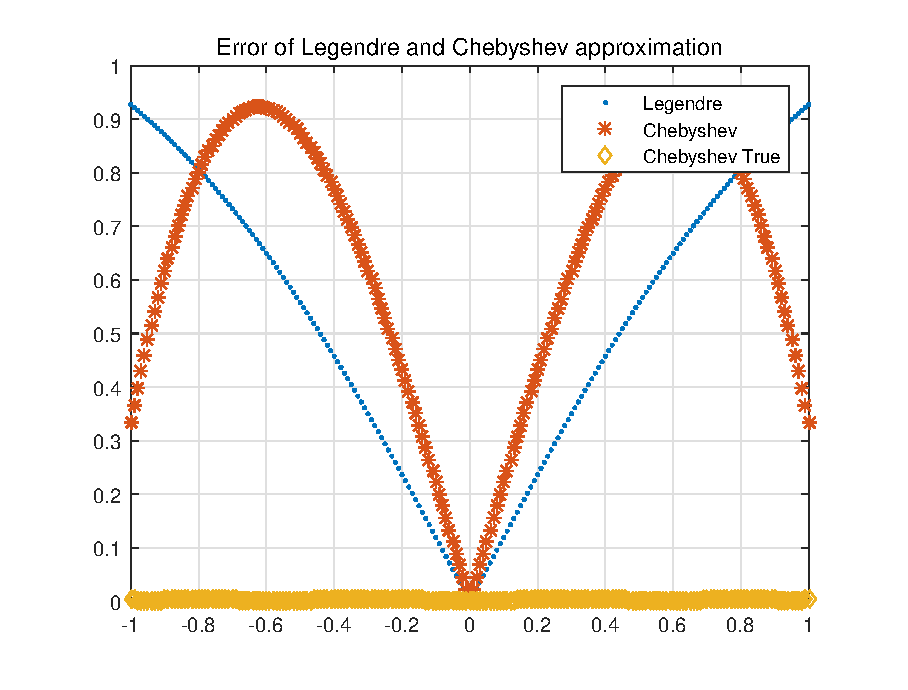
\includegraphics[width = 10cm]{prob1.eps}

Use the result of True Chebyshev approximation $\hat{t_3}(x)$, we can find maximum of errors satisfying Theorem 9: \\
\begin{tabular}{|c|c|}
\hline
x & error \\
\hline
-1.0 & -0.004 \\
\hline
-0.86 & 0.004 \\
\hline
-0.38 & -0.004 \\
\hline
0.39 & 0.004 \\
\hline
0.88 & -0.004 \\
\hline
1.0 & 0.004 \\
\hline
\end{tabular}

And the maxima of error using True Chebyshev approximation is 0.0047, it shows
$$
0.004 \le \rho_3(f) \le 0.0047.
$$
}

\problem{2}{Problem 4.31}
\solution{code}{
By Lagrange form, we can compute the near minimax approximations using the code:
}
\lstinputlisting[language = MATLAB]{near_minimax.m}
\lstinputlisting[language = MATLAB]{prob2.m}
\solution{Result}{
The graph of error, and the max error of infinite norm are as below, and for each $n$ and function $f$, using Theorem 4.9, $\rho_n(f)$ is less or equal than the infinite norm of error. The left bound is just too difficult to find.
}
\begin{figure}
\centering
\begin{minipage}{0.45\textwidth}
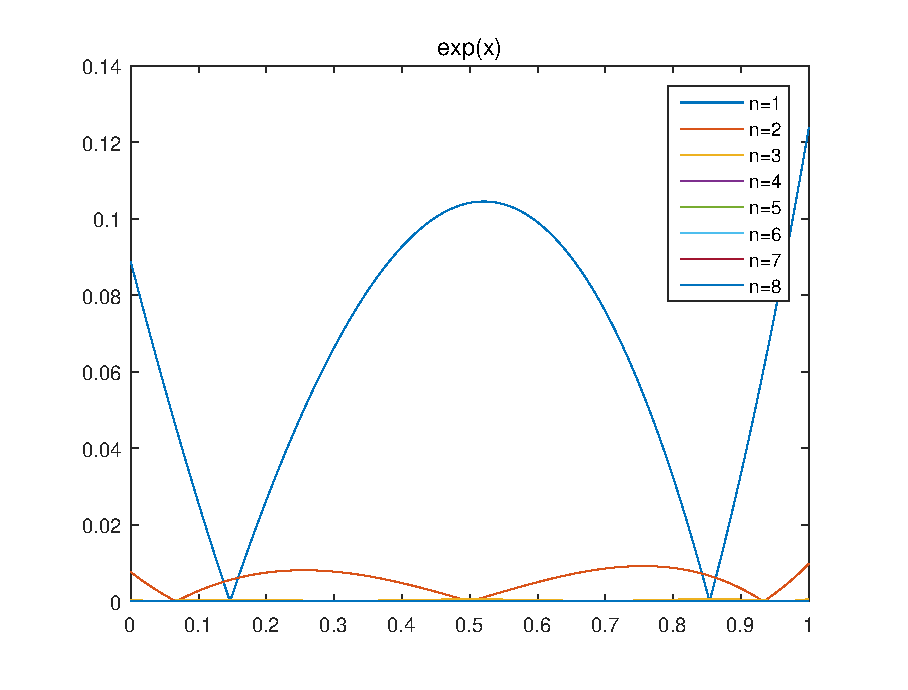
\includegraphics[width = \textwidth]{prob2a.eps}
\end{minipage}
\begin{minipage}{0.45\textwidth}
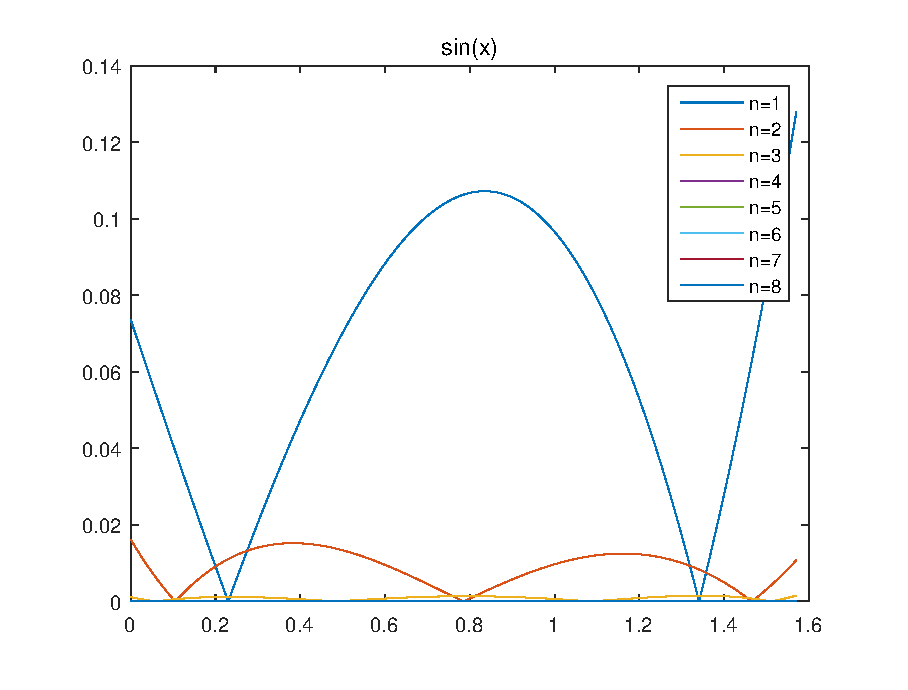
\includegraphics[width = \textwidth]{prob2b.eps}
\end{minipage} \\
\begin{minipage}{0.45\textwidth}
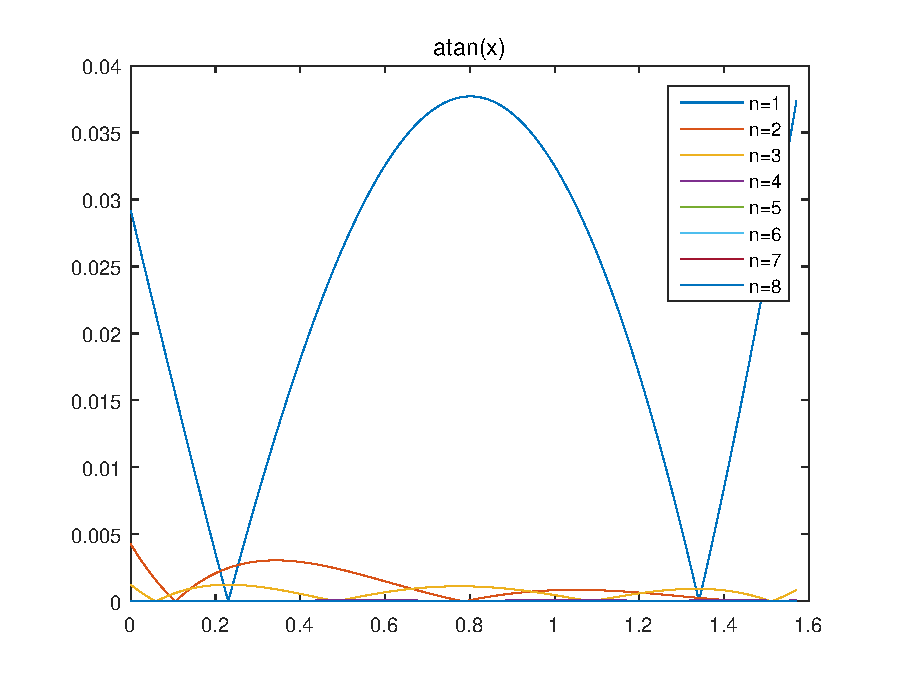
\includegraphics[width = \textwidth]{prob2c.eps}
\end{minipage}
\begin{minipage}{0.45\textwidth}
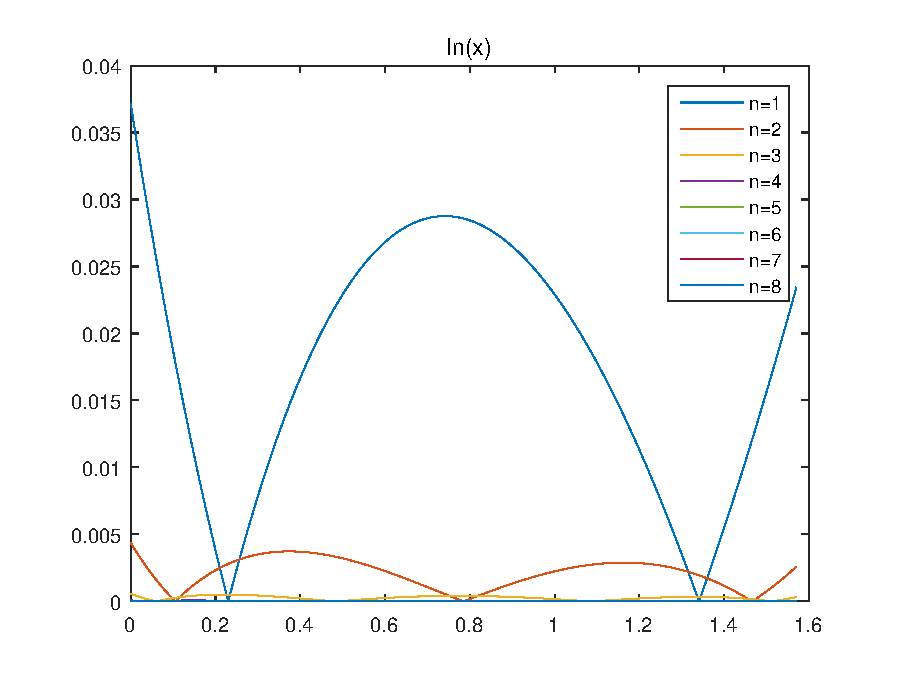
\includegraphics[width = \textwidth]{prob2d.eps}
\end{minipage}
\end{figure}
\begin{lstlisting}[language = MATLAB]
error1 =

   0.123795135763495
   0.009865548570435
   0.000600007042634
   0.000029454776569
   0.000001211208768
   0.000000042830298
   0.000000001328131
   0.000000000036665

error2 =

   0.128085593199313
   0.016221586055544
   0.001558351287206
   0.000120525677443
   0.000007798442861
   0.000000433620299
   0.000000021134835
   0.000000000916854

error3 =

   0.037696680264831
   0.004285211299804
   0.001249669440946
   0.000128958381678
   0.000031926143639
   0.000006935414046
   0.000000610998106
   0.000000258964760

error4 =

   0.037165432256798
   0.004372493413419
   0.000572167228374
   0.000079420776488
   0.000011447097561
   0.000001693662660
   0.000000255467302
   0.000000039109056
\end{lstlisting}


\problem{3}{Problem 4.34}
\solution{Sol}{
$$
\begin{aligned}
f(x)-I_n(x) &= f(x)-C_n(x)+C_n(x)-I_n(x) = f(x)-C_n(x)-\sum_{j=0}^{n}(f(x_j)-C_n(x_j))l_j(x) \\
&= g(x)-\sum_{j=0}^{n}g(x_j)l_j(x),
\end{aligned}
$$
where
$$
g(x) = f(x)-C_n(x) = c_{n+1}T_{n+1}(x)+\sum_{j = n+2}^{\infty}c_jT_j(x).
$$
Since $x_j$ are roots of $T_{n+1}(x)$, and 
$$
\sum_{j = n+2}^{\infty}c_jT_j(x) \ll c_{n+1}T_{n+1}(x),
$$
then there exists $\alpha_n,~\beta_n $, s.t. 
$$
\alpha_n|T_{n+1}| \le |f-I_n| \le \beta_n|T_{n+1}|.
$$
Using (4.7.28),
$$
\rho_n(f)\le \lVert f-I_n\rVert_{\infty} \le\frac{1}{(n+1)!2^n}\lVert f^{(n+1)}\rVert_{\infty} \le \frac{1}{(n+1)!2^n}.
$$
On the other hand, using (4.7.30),
$$
\rho_n(f) \ge \frac{1}{2+\frac{2}{\pi}\log(n+1)}\lVert f-I_n\rVert_{\infty} \ge \frac{\alpha_n}{2+\frac{2}{\pi}\log(n+1)} \max |T_{n+1}| = \frac{\alpha_n}{2+\frac{2}{\pi}\log(n+1)}.
$$
}

\problem{4}{Problem 4.37}
\solution{Sol}{
We can get the result from (4.7.48) and (4.7.39). Denote $f(x) = x^6-x^3$.

When $n = 0$,
$$
x_0 = 1, ~x_1 = -1, ~E_0 = \frac{1}{2}(f(x_0)-f(x_1)) = -1.
$$
When $n = 1$,
$$
x_0 = 1, ~x_1 = 0, ~x_2 = -1, ~E_1 = \frac{1}{2}(\frac{1}{2}(f(x_0)+f(x_2))-f(x_1)) = \frac{1}{2}.
$$
When $n = 2$,
$$
x_0 = 1, ~x_1 = \frac{1}{2}, ~x_2 = -\frac{1}{2}, ~x_3 = -1, ~E_2 = \frac{1}{3}(\frac{1}{2}(f(x_0)-f(x_3))-f(x_1)+f(x_2)) = -\frac{1}{4}.
$$
When $n = 3$,
$$
x_0 = 1, ~x_1 = \frac{\sqrt{2}}{2}, ~x_2 = 0, ~x_3 = -\frac{\sqrt{2}}{2}, ~x_4 = -1, ~E_3 = \frac{1}{4}(\frac{1}{2}(f(x_0)+f(x_4))-f(x_1)+f(x_2)-f(x_3)) = \frac{3}{16}.
$$
When $n = 4$,
$$
x_0 = 1, ~x_1 = \cos(\pi/5), ~x_2 = \cos(2\pi/5), ~x_3 = \cos(3\pi/5), ~x_4 = \cos(4\pi/5), ~x_5 = -1,
$$
$$
E_4 = \frac{1}{5}(\frac{1}{2}(f_0-f_5)-f_1+f_2-f_3+f_4) = 0.
$$
When $n = 5$,
$$
x_0 = 1, ~x_1 = \frac{\sqrt{3}}{2}, ~x_2 = \frac{1}{2}, ~x_3 = 0, ~x_4 = -\frac{1}{2}, ~x_5 = \frac{\sqrt{3}}{2}, ~x_6 = -1,
$$
$$
E_5 = \frac{1}{6}(\frac{1}{2}(f_0+f_6)-f_1+f_2-f_3+f_4-f_5) = \frac{1}{32}.
$$
Thus
$\alpha = 0$, and
$$
c_{4, 0} = \frac{2}{5}(\frac{1}{2}(f_0\cos0+f_5\cos0) + f_1\cos0+f_2\cos0+f_3\cos0+f_4\cos0) = \frac{5}{8},
$$
$$
c_{4, 1} = \frac{2}{5}(\frac{1}{2}(f_0\cos0+f_5\cos\pi)+f_1\cos(\pi/5)+f_2\cos(2\pi/5)+f_3\cos(3\pi/5)+f_4\cos(4\pi/5)) = -\frac{3}{4},
$$
$$
c_{4, 2} = \frac{2}{5}(\frac{1}{2}(f_0\cos0+f_5\cos2\pi)+f_1\cos(2\pi/5)+f_2\cos(4\pi/5)+f_3\cos(6\pi/5)+f_4\cos(8\pi/5)) = \frac{15}{32},
$$
$$
c_{4, 3} = \frac{2}{5}(\frac{1}{2}(f_0\cos0+f_5\cos3\pi)+f_1\cos(3\pi/5)+f_2\cos(6\pi/5)+f_3\cos(9\pi/5)+f_4\cos(12\pi/5)) = -\frac{1}{4},
$$
$$
c_{4, 4} = \frac{2}{5}(\frac{1}{2}(f_0\cos0+f_5\cos4\pi)+f_1\cos(4\pi/5)+f_2\cos(8\pi/5)+f_3\cos(12\pi/5)+f_4\cos(16\pi/5)) = \frac{7}{32}
$$
$$
c_{4, 5} = \frac{2}{5}(\frac{1}{2}(f_0\cos0+f_5\cos5\pi)+f_1\cos(5\pi/5)+f_2\cos(10\pi/5)+f_3\cos(15\pi/5)+f_4\cos(20\pi/5)) = 0.
$$
Thus
$$
p_5(x) = \frac{5}{8} -\frac{3}{4}x+\frac{15}{32}(2x^2-1)-\frac{1}{4}(4x^3-3x)+\frac{7}{32}(8x^4-8x^2+1) = \frac{7}{4}x^4-x^3-\frac{13}{16}x^2+\frac{3}{8}.
$$
}


\end{document}